\titlespacing*{\subsection}
  {0pt}{2\baselineskip}{\baselineskip}

\chapter{Introducción}

La renderización es el proceso de generar una imagen a partir de la descripción de una escena 2D o 3D. Dicho proceso puede ser abordado de muchas formas, siendo nuestro objeto de estudio los renderizadores físicamente realistas que utilizan el algoritmo de \emph{ray-tracing}, denominados \emph{ray tracers}. Los renderizadores físicamente realistas o fotorrealistas utilizan los principios de la física para modelar el comportamiento de la luz y su interacción con la materia. En este capítulo se presentará el algoritmo de ray-tracing y su fundamentación física y matemática, así como también se describirá brevemente el concepto de método de Monte Carlo y su uso dentro de los ray-tracers. Posteriormente se establecerán los contenidos de este trabajo, comentando las fuentes utilizadas.

\section{El algoritmo de ray-tracing}

El objetivo de los renderizadores fotorrealistas es crear imágenes de escenas 3D que simulen la realidad de la manera más fiel posible, es decir, buscan generar imágenes que parezcan fotografías reales. La mayor parte de renderizadores fotorrealistas utilizan ray-tracing, un algoritmo que consiste en simular el camino que siguen los rayos de luz a través de la escena para poder así determinar el color de cada píxel de la imagen final. Este enfoque más realista de la renderización empezó a cobrar importancia durante la década de 1980, con el artículo \cite{Whitted}, que introdujo la idea de usar ray-tracing para el cálculo de la distribución de la luz en escenas 3D. Desde entonces se han detallado numerosos modelos enfocados a la síntesis realista de imágenes. Destacar también la importancia de \cite{Kajiya86}, que presentó una solución al problema del cálculo de iluminación global a través de un modelo riguroso basado en la ecuación de renderización, mostrando una forma de aproximar dicha ecuación mediante el uso de métodos de Monte Carlo, y \cite{Veach97}, que desarrolló nuevos algoritmos para ray-tracing basados en métodos de Monte Carlo.

Vamos por tanto a detallar los aspectos más relevantes del algoritmo de ray-tracing, siguiendo las ideas detalladas en el libro \cite{Pharr2016}. Hay una serie de objetos y fenómenos que todos los ray tracers deben ser capaces de simular de manera más o menos realista: la cámara desde la que se visualiza la escena, la intersección de rayos con objetos de la escena, la visibilidad de las fuentes de luz desde un punto de la escena, la distribución de la cantidad de luz reflejada y transmitida por la superficie de los objetos (\emph{surface scattering}), la distribución de la luz en la escena y la propagación de los rayos a través de medios diferentes al vacío.
\subsection{Cámara}

Si queremos generar una imagen realista necesitamos simular el funcionamiento de una cámara real, y la forma en que modelemos la cámara determinará el modo en que la escena es vista. El modelo de cámara más simple utilizado en ray-tracing está basado en la cámara estenopeica, una cámara sin lente consistente en una caja con un pequeño agujero por el que entra la luz y un trozo de papel fotográfico donde queda grabada la imagen.

\begin{figure}[h]
  \lineskip=-\fboxrule
  \fbox{\begin{minipage}{\dimexpr \textwidth-2\fboxsep-2\fboxrule}
    \centering
    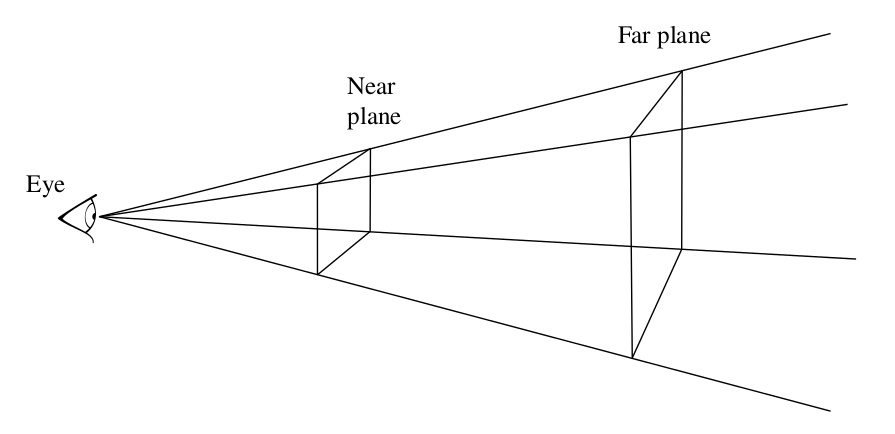
\includegraphics[width=0.7\textwidth]{imagenes/figura1_1}
  \end{minipage}}
  \fbox{\begin{minipage}{\dimexpr \textwidth-2\fboxsep-2\fboxrule}
    \abovecaptionskip=0pt
    \caption{Simulación de la cámara estenopeica.}
    \source{\cite{Pharr2016}}
  \end{minipage}}
\end{figure}

La cámara estenopeica puede ser simulada haciendo una abstracción y suponiendo que el papel de película se encuentra a cierta distancia en la dirección en la que la cámara está apuntando. Tal y como podemos ver en la figura 1.1, uniendo la posición dónde se encuentra la cámara con los filos de la película (near plane) se obtiene una región del espacio con forma de pirámide, que será la región del espacio que será captada en la imagen final. Sin embargo falta determinar que color tendrá la imagen en cada uno de sus píxeles. Para ello se traza un número concreto de rayos que pasan por cada píxel y a continuación se calcula la cantidad de luz que viaja a través de cada rayo trazado, lo cual constituye el principal problema a resolver dentro de los ray tracers. Por último se hace una media de los rayos que pasan por cada píxel para calcular su color.

El modelo de cámara recién presentado, a pesar de ser muy usado dentro de la renderización por ordenador, está bastante alejado del funcionamiento de una cámara actual, por lo que es deseable un modelo más complejo dentro de un renderizador fotorrealista. Esto se consigue simulando la utilización de múltiples lentes que nos permiten conseguir diversos efectos en la imagen final. Por otro lado, es común utilizar un parámetro temporal asociado a los rayos trazados, trazando varios rayos a lo largo del tiempo. La posición de los objetos de la escena puede cambiar en el tiempo, con lo que de esta manera se puede simular que ciertos objetos estén en movimiento al momento de tomar la fotografía. 


Aunque puedan utilizarse modelos de cámara más complejos, todos estos modelos coinciden en que su principal tarea es determinar el espacio dentro de la escena que será captado en la imagen y trazar los rayos correspondientes a cada píxel.

\subsection{Intersección de rayos con objetos de la escena}

Una vez los rayos son trazados por la cámara, estos interseccionarán con objetos de la escena. La primera tarea del renderizador es ser capaz de calcular el punto en que cada rayo intersecciona con la escena, así como calcular las propiedades geométricas locales del objeto interseccionado.

\subsection{Visibilidad}

Recordemos que el objetivo es calcular la cantidad de luz que viaja por cada rayo que llega a la película de la cámara, o lo que es lo mismo, si consideramos el punto dónde el rayo intersecciona con la escena, calcular la cantidad de luz que viaja desde dicho punto en dirección a la cámara. Este proceso que se utiliza para calcular el color que se percibe de un punto de la escena se conoce como \emph{sombreado} o \emph{shading}.

Para calcular la cantidad de luz que es reflejada desde un punto en una dirección, primero es necesario estimar la cantidad de luz que llega a él. Por tanto es esencial que el renderizador sea capaz de determinar si una fuente de luz es visible desde el punto de la escena que está siendo sombreado.

\subsection{Distribución de la dispersión de la luz en superficies}

Llegados a este punto vemos que la forma en que los objetos de la escena reflejan y transmiten la luz que les llega es de gran importancia. Esto depende de las características de la materia que compone el objeto. La función que describe la forma en que los objetos de la escena reflejan la luz que reciben se denomina \emph{función de distribución de reflectancia bidireccional} o \emph{BRDF} (\emph{bidirectional reflectance distribution function}), y la notaremos por:
$$f_r:\mathds{R}^3\times \mathds{S}^2 \times \mathds{S}^2 \rightarrow \mathds{R}^+_0$$

Dónde notamos por $\mathds{S}^2$ a la esfera unidad de $\mathds{R}^3$. De esta manera, sea $p$ un punto en la superficie de un objeto, $\omega _i$ la dirección de un rayo incidente, y $\omega _o$ la dirección de un rayo reflejado, entonces la cantidad de energía reflejada por la superficie del objeto en el punto $p$ desde la dirección $\omega _i$ hacia la dirección $\omega _o$ es $f_r(p,\omega _o, \omega _i)$. Obviamente al tratarse de energía reflejada, si consideramos la esfera cuyo polo norte es la normal en $p$ a la superficie (notada como $n$ en la figura 1.2), si $\omega _i$ se encuentra en el hemisferio inferior de dicha esfera entonces $f_r(p,\omega _o, \omega _i)$ será igual a 0.\\

\begin{figure}[h]
  \lineskip=-\fboxrule
  \fbox{\begin{minipage}{\dimexpr \textwidth-2\fboxsep-2\fboxrule}
    \centering
    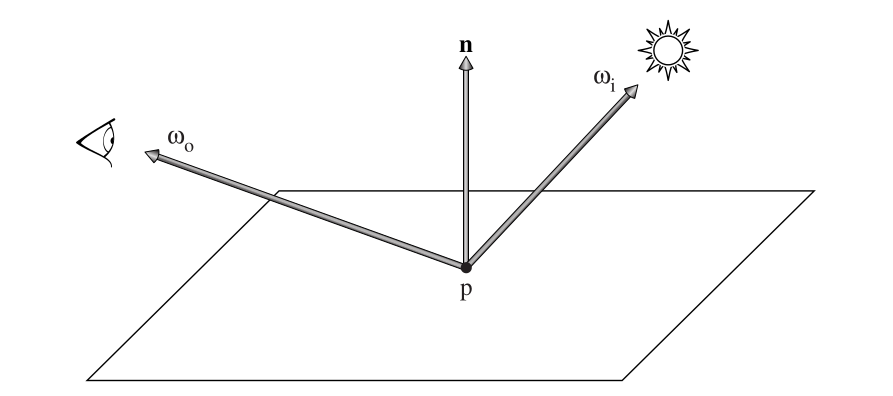
\includegraphics[width=0.7\textwidth]{imagenes/figura1_2}
  \end{minipage}}
  \fbox{\begin{minipage}{\dimexpr \textwidth-2\fboxsep-2\fboxrule}
    \abovecaptionskip=0pt
    \caption{Reflexión de la luz}
    \source{\cite{Pharr2016}}
  \end{minipage}}
\end{figure}

De manera similar podemos definir la función que describe la cantidad de energía transmitida, es decir, la cantidad de energía que atraviesa el objeto y escapa en una dirección. A dicha función la llamaremos \emph{función de distribución de transmitancia bidireccional} o \emph{BTDF} (\emph{bidireccional tramittance distribution function}) y la notamos por $f_t$.

Por último consideramos la función que describe de manera conjunta la energía reflejada y transmitida, la \emph{función de distribución de dispersión bidireccional} o \emph{BSDF} (\emph{bidirectional scattering distribution function}) que notamos por $f$.

En el caso de un objeto que presente reflexión especular perfecta, el BSDF en su superficie se puede describir de manera sencilla, ya que dada una dirección $\omega _i$, toda la luz procedente de esa dirección será reflejada en una única dirección saliente $\omega _o$, que será aquella que forme el mismo ángulo con la normal a la superficie que $\omega _i$. Este sería el caso de un espejo perfecto. Sin embargo la mayor parte de objetos de la vida real no se comportan de esta manera, por lo que en un ray tracer habrá diversos modelos que simulen diferentes materiales.

\subsection{Distribución de la luz}

La radiometría y la óptica geométrica nos otorgan las herramientas físicas y matemáticas que necesitamos para describir el comportamiento de la luz, y forman la base de la mayor parte de algoritmos utilizados en ray-tracing. La radiometría es la ciencia que trata la medición de radiación electromagnética, ya sea visible o no. La óptica geométrica tiene en cuenta propiedades macroscópicas de la luz, que son suficientes para describir la forma en que la luz interacciona con objetos mucho más grandes que su longitud de onda. Por otra parte, no es raro simular fenómenos propios de la óptica física, aunque en nuestro caso no tendremos en cuenta este tipo de fenómenos. Hay una serie de asunciones que haremos acerca del comportamiento de la luz para simplificar el cálculo de la energía radiante en la escena:

\begin{itemize}
\item Linealidad: El efecto combinado de dos entradas en un sistema óptico es siempre igual a la suma del efecto de cada una de las entradas individualmente.
\item Conservación de la energía: La energía radiante reflejada o transmitida por una superficie nunca será mayor que la energía incidente sobre dicha superficie.
  \item Estado de reposo: Se asume que la distribución de la luz en la escena ha alcanzado el equilibrio, por lo que no habrá cambios en la distribución de la radiancia a lo largo del tiempo.
\end{itemize}

Antes de presentar las magnitudes radiométricas centrales en renderización, vamos a definir el concepto de \emph{ángulo sólido}.

\subsubsection*{Ángulo sólido}

Como ya sabemos, en una circunferencia de radio unidad, el ángulo en radianes entre dos radios es igual a la longitud de circunferencia comprendida entre ellos (figura 1.3). Conceptualmente, el ángulo sólido se trata de una extensión de los ángulos planos a $\mathds{R}^3$, y mide el tamaño con el que se ve un objeto desde un punto. Podemos entender un objeto como una superficie simple, regular a trozos y orientable.

\begin{definicion}
    Sea $P \in \mathds{R}^3$ y consideremos la esfera unidad con centro $P$, $\mathcal{B}(P,1)$. Sea $\pi :\mathds{R}^3/\{P\}\rightarrow \mathcal{B}(P,1)$ la proyección sobre la esfera $\mathcal{B}(P,1)$, es decir, $\pi(r) = P + \frac{r-P}{\|r-P\|}$. Sea $A \subseteq \mathds{R}^3/\{P\}$ una superficie simple, regular a trozos y orientable, y tomamos $I = \int _{\pi(A)} dS$. Entonces diremos que el ángulo sólido subtendido por $A$ desde $P$ mide $I$ estereorradianes.
\end{definicion}

\begin{figure}[h]
  \lineskip=-\fboxrule
  \fbox{\begin{minipage}{\dimexpr \textwidth-2\fboxsep-2\fboxrule}
    \centering
    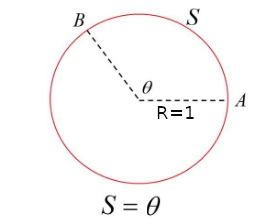
\includegraphics[width=0.3\textwidth]{imagenes/figura1_5}
  \end{minipage}}
  \fbox{\begin{minipage}{\dimexpr \textwidth-2\fboxsep-2\fboxrule}
    \abovecaptionskip=0pt
    \caption{Ángulo plano}
  \end{minipage}}
\end{figure}

\begin{figure}[h]
  \lineskip=-\fboxrule
  \fbox{\begin{minipage}{\dimexpr \textwidth-2\fboxsep-2\fboxrule}
    \centering
    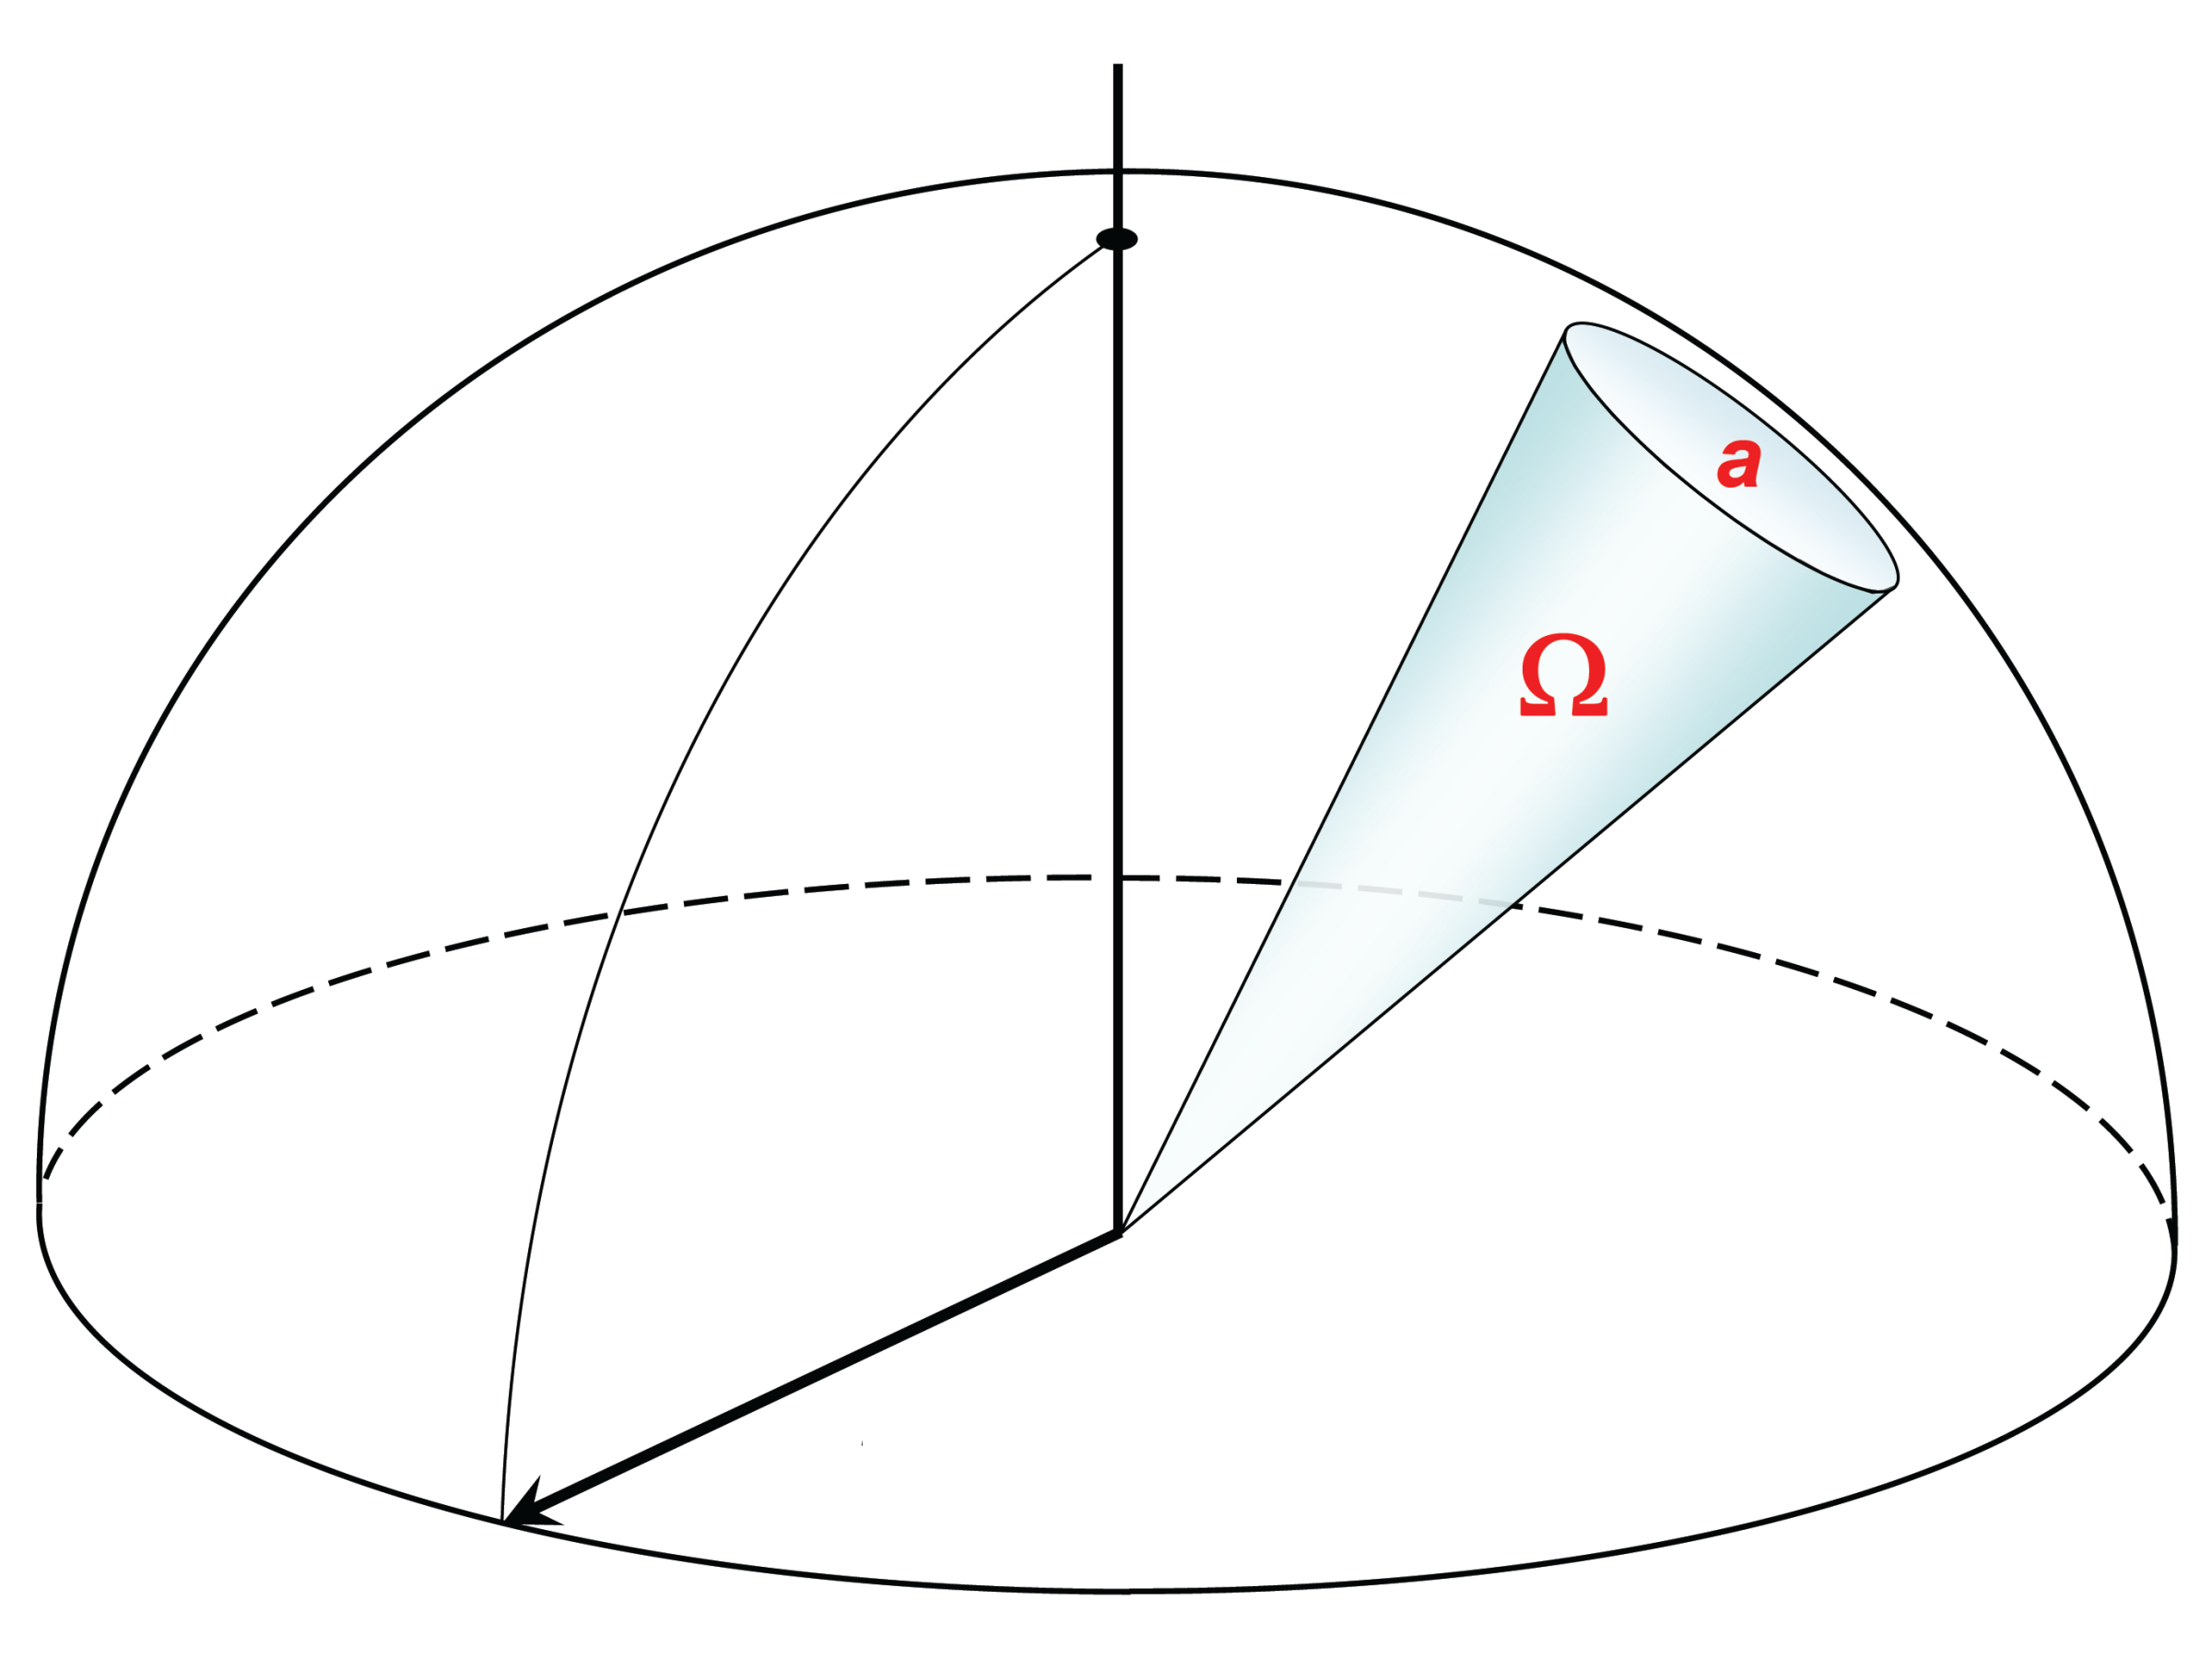
\includegraphics[width=0.6\textwidth]{imagenes/figura1_4}
  \end{minipage}}
  \fbox{\begin{minipage}{\dimexpr \textwidth-2\fboxsep-2\fboxrule}
    \abovecaptionskip=0pt
    \caption{Ángulo sólido}
  \end{minipage}}
\end{figure}

En la definición anterior hemos usado $dS$ para denotar la integral de superficie. Como vemos el ángulo sólido subtendido por un objeto claramente depende del punto de referencia $P$. Sin embargo, supongamos que queremos medir el ángulo sólido subtendido por un objeto desde un punto $P$. En renderización se trabaja con $\mathds{R}^3$ como espacio afín, por lo que podemos aplicar una traslación del marco de referencia para situar $P$ en el origen de coordenadas. Por tanto, a efectos prácticos siempre podemos suponer que trabajamos en la esfera unidad $\mathds{S}^2$. Vamos a definir ahora la función que mide el ángulo sólido en la esfera unidad:

\begin{definicion}
  Sea $\mathscr{S}$ la familia de superficies contenidas en la esfera unidad $\mathds {S}^2$, definimos la función $\mu :\mathscr{S} \rightarrow \mathds{R}^+_0$ como:
  $$\mu(C) = \int_C \text{ }dS , \hspace{0.5cm} \forall C\in \mathscr{S}$$

  La función $\mu$ mide el ángulo sólido subtendido por cada superficie simple de la esfera.
\end{definicion}

Vamos ahora a derivar una serie de resultados básicos relacionados con el ángulo sólido que nos serán útiles durante el resto del trabajo. Consideremos la parametrización de la esfera unidad $\Theta:[0,\pi ]\times [0,2\pi ]\rightarrow \mathds{R}^3$, con:
$$\Theta(\theta ,\varphi ) = ( \sin \theta \cos \varphi,  \sin \theta \sin \varphi , \cos \theta),\hspace{0.5cm}  \forall (\theta , \varphi)\in [0,\pi ]\times [0,2\pi ]$$

Derivando parcialmente $\Theta$ y calculando el producto vectorial de sus derivadas parciales vemos que:
$$\Theta _\theta(\theta ,\varphi ) = \frac{\partial \Theta}{\partial \theta}(\theta ,\varphi ) = (\cos\theta\cos\varphi, \cos\theta\sin\varphi, -\sin\theta)$$

$$\Theta _\varphi(\theta ,\varphi ) = \frac{\partial \Theta}{\partial \varphi}(\theta ,\varphi ) = (-\sin\theta\sin\varphi, \sin\theta\cos\varphi, 0)$$

$$\Theta _\theta(\theta ,\varphi )\times \Theta _\varphi(\theta ,\varphi ) = (\sin^2\theta\cos\varphi,\sin^2\theta\sin\varphi,\sin\theta\cos\theta)$$

Con lo que concluimos que:
\begin{align}\label{intAngSolSin}
\begin{split}
\mu (C) = \int_C \text{ }dS &= \iint_{\Theta^{-1}(C)}\|\Theta _\theta(\theta ,\varphi )\times \Theta _\varphi(\theta ,\varphi )\| d\theta d\varphi \\
&= \iint_{\Theta^{-1}(C)} \sin\theta d\theta d\varphi \hspace{1cm} \forall C \in \mathscr{S}
\end{split}
\end{align}

De aquí en adelante, por comodidad, notaremos por $\pi$ a la proyección sobre la esfera unidad $\mathds{S}^2$, es decir, $\pi(p)=\frac{p}{\|p\|}$, $\forall p \in \mathds{R}^3/\{(0,0,0)\}$. Pasamos ahora a demostrar la siguiente proposición:

\begin{proposicion}\label{angSolido1}
  Sea $\mu$ la medida del ángulo sólido, y sea $C$ una superficie en $\mathds{R}^3/\{(0,0,0)\}$ simple, regular a trozos y orientable, tal que cada recta que empiece en el origen y acabe en un punto de $C$ sólo interseccione con $C$ una vez. Consideramos la función $g:\mathds{R}^3/\{(0,0,0)\} \rightarrow \mathds{R}^3$, con $g(p)=\frac{p}{\|p\|^3}$. Entonces se cumple que:

 \begin{equation}
 \mu (\pi(C)) = \int _C g \text{ }dS 
 \end{equation}
 
\end{proposicion}

\begin{figure}[h]
  \lineskip=-\fboxrule
  \fbox{\begin{minipage}{\dimexpr \textwidth-2\fboxsep-2\fboxrule}
    \centering
    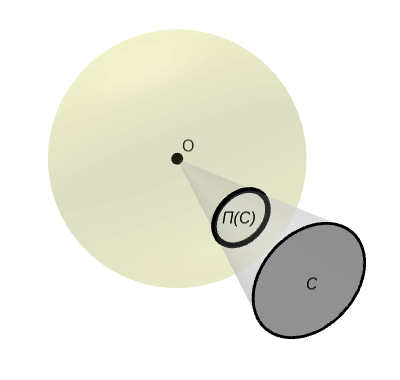
\includegraphics[width=0.6\textwidth]{imagenes/figura1_6}
  \end{minipage}}
  \fbox{\begin{minipage}{\dimexpr \textwidth-2\fboxsep-2\fboxrule}
    \abovecaptionskip=0pt
    \caption{Medida del ángulo sólido de una superficie simple y regular a trozos}
  \end{minipage}}
\end{figure}

\begin{notacion}
Notaremos por $u \cdot v$ al producto escalar de los vectores $u$ y $v$.
\end{notacion}

\begin{proof}

Sea $C_r$ la porción del espacio comprendida entre $C$ y $\pi (C)$, y sea $\partial C_r$ su frontera. Sea $C_p = \partial C_r /(C\cup \pi(C))$ la superficie que delimita lateralmente la región $C_r$. Vamos ahora a calcular la divergencia de $g$. Sea $(x,y,z)\in \mathds{R}^3$:

\begin{align*}
  \textrm{div } g (x,y,z) &= \frac{\partial g}{\partial x}(x,y,z) + \frac{\partial g}{\partial y}(x,y,z) + \frac{\partial g}{\partial z} (x,y,z) =\\
  & = \frac{(x^2+y^2+z^2)^{\frac{3}{2}}-3x^2(x^2+y^2+z^2)^{\frac{1}{2}}}{(x^2+y^2+z^2)^3} +\\
  & + \frac{(x^2+y^2+z^2)^{\frac{3}{2}}-3y^2(x^2+y^2+z^2)^{\frac{1}{2}}}{(x^2+y^2+z^2)^3} +\\
  &+ \frac{(x^2+y^2+z^2)^{\frac{3}{2}}-3z^2(x^2+y^2+z^2)^{\frac{1}{2}}}{(x^2+y^2+z^2)^3} = 0
\end{align*}

Y, por tanto, aplicando el teorema de divergencia tenemos que:

$$\int _{\partial C_r}g\text{ } dS = \iiint _{C_r}\text{div } g \text{ }dx dy dz = 0$$

Sea $C_p = \bigcup _{i=1}^n S_i$ una descomposición finita de $C_p$ como unión de superficies simples y regulares. Fijado $i\in \{1\ldots n\}$, sea $\Psi^i : W^i \rightarrow \mathds{R}^3$ una parametrización simple y suave de $S_i$ orientada mediante la normal exterior, y sean $\Psi^i_u$, $\Psi^i_v$ sus derivadas parciales. Es fácil ver que dado un punto $P\in S_i$, se tiene que el vector que va desde el origen hasta $P$ es perpendicular a la normal a $S_i$ en $P$. Por tanto tenemos que:

$$ \int_{S_i} g\text{ }dS = \iint _{W^i} \frac{\Psi^i(u,v) \cdot (\Psi^i_u(u,v)\times \Psi^i_v (u,v))}{\|\Psi^i(u,v)\|^3}\text{ } du dv = 0$$


Dónde se ha usado que $\Psi^i(u,v) \cdot (\Psi^i_u(u,v)\times \Psi^i_v (u,v)) = 0$, $\forall (u,v)\in W^i$, ya que el producto vectorial de las derivadas parciales es igual a la normal a la superficie y el producto escalar de vectores perpendiculares es nulo. Sabemos que $\partial C_i = C\cup \pi(C) \cup C_p$, y usando las dos igualdades anteriores tenemos que:

$$0 = \int _{\partial C_r}g\text{ } dS = \int _{C}g\text{ } dS + \int _{\pi(C)}g\text{ } dS $$

Sea $\Phi :W\rightarrow \mathds{R}^3$, una parametrización simple y suave de $\pi (C)$ orientada con la normal exterior, y sean $\Phi _u$, $\Phi _v$ sus derivadas parciales. Como $\pi (C)$ está contenido en la esfera unidad, para todo $(u,v)\in W$ se cumple que $-\Phi(u,v) = \frac{\Phi_u(u,v)\times \Phi_v (u,v)}{\|\Phi_u(u,v)\times \Phi_v (u,v)\|}$ y que  $\|\Phi(u,v)\| = 1$, y por ello:

\begin{align*}
  \int _{\pi(C)}g\text{ } dS &= \iint _{W} \frac{\Phi(u,v) \cdot (\Phi_u(u,v)\times \Phi_v (u,v))}{\|\Phi(u,v)\|^3}\text{ } du dv =\\
  &= - \iint _{W} \frac{\|\Phi_u(u,v)\times \Phi_v (u,v)\|}{\|\Phi(u,v)\|^2}\text{ } du dv = - \int _{\pi(C)}\text{ } dS
\end{align*}

Y por tanto deducimos que:

\begin{align*}
  & 0 = \int _{C}g\text{ } dS + \int _{\pi(C)}g\text{ } dS = \int _{C}g\text{ } dS - \int _{\pi(C)}\text{ } dS \Rightarrow \\
  & \Rightarrow \int _{C}g\text{ } dS = \int _{\pi(C)}\text{ } dS = \mu (\pi(C))
\end{align*}

Tal y como queríamos.\\
\end{proof}

Podemos ahora introducir un concepto bastante natural por la forma en que hemos definido la función $\mu$.

\begin{definicion}
  Sea $C\subseteq \mathds{S}^2$ una superficie simple y sea $h: C\rightarrow \mathds{R}$ un campo escalar, $i: C\rightarrow \mathds{R}^3$ un campo vectorial. Entonces la integral respecto al ángulo sólido de las funciones $h$ e $i$ se define como:

  $$\int _C h\text{ } d\mu = \int _C h\text{ } dS$$

   $$\int _C i\text{ } d\mu = \int _C i\text{ } dS$$
  
\end{definicion}

Y por último podemos generalizar la proposición \ref{angSolido1} de la siguiente manera:

\begin{proposicion}\label{ToArea}
Sea $C$ una superficie en $\mathds{R}^3/\{(0,0,0)\}$ simple, regular a trozos y orientable, tal que cada recta que empiece en el origen y acabe en un punto de $C$ sólo interseccione con $C$ una vez. Sea $h: \mathds{S}^2\rightarrow \mathds{R}^+_0$ un campo escalar no negativo. Consideramos la función $g:\mathds{R}^3/\{(0,0,0)\} \rightarrow \mathds{R}^3$, con $g(p)=\frac{p}{\|p\|^3}$. Entonces se cumple que:

 \begin{equation}\label{transfToArea}
   \int_{\pi(C)} h\text{ }d\mu = \int _C (h\circ \pi) g \text{ }dS 
 \end{equation}
 
  \end{proposicion}

\subsubsection*{Medida de la luz}

Una vez nos hemos familiarizado con el concepto de ángulo sólido, vamos a presentar una serie de magnitudes radiométricas básicas. Todas estas magnitudes dependen de la longitud de onda, y aunque obviaremos esto, es importante tenerlo en cuenta.

\begin{itemize}
\item \textbf{Energía radiante}: Las fuentes de luz emiten fotones, cada uno de los cuales porta una cantidad de energía que depende de la longitud de onda. La energía se mide en julios (j), y notaremos por $Q$ a la función que mide la energía en una región durante un periodo de tiempo.
\item \textbf{Flujo radiante}: La energía está medida sobre algún periodo de tiempo, y por tanto, bajo la asunción de estado de reposo, es más conveniente trabajar con magnitudes que se midan en un instante de tiempo. El flujo radiante se define como la cantidad total de energía por unidad de tiempo que atraviesa una región. Se mide en vatios (W), y notaremos por $\Phi$ a la función que mide el flujo radiante en una región.
\item \textbf{Irradiancia y emitancia radiante}: Las dos magnitudes miden el flujo radiante por unidad de superficie, en el caso de la irradiancia se mide el flujo llegando a la superficie, y en el caso de la emitancia radiante se mide el flujo saliendo de la superficie. Se mide en vatios por metro cuadrado (W/m$^{-2}$) y notaremos por $E$ a la función que mide la irradiancia.

\item \textbf{Radiancia incidente y saliente}: Se trata de la magnitud que más utilizaremos. La irradiancia nos da una medida del flujo radiante por unidad de superficie, pero no tiene en cuenta que el flujo tiene una distribución direccional, es decir, la cantidad de flujo que llega a una superficie varía según la dirección del flujo incidente. La radiancia mide el flujo por unidad de superficie proyectada y por unidad de ángulo sólido. Cuando hablamos de superficie proyectada nos referimos a que calculamos el flujo en una superficie hipotética que es perpendicular a la dirección del flujo incidente/saliente. Se mide en vatios por estereorradián por metro cuadrado (W sr$^{-1}$ m$^{-2}$) y notaremos por $L: \mathds{R}^3 \times \mathds{S}^2\rightarrow \mathds{R}^+_0$ a la función que mide la radiancia.

  Notemos por $\mathcal{H}^2(n)$ al hemisferio superior de la esfera unidad cuyo polo norte es el vector $n$. Si consideramos una superficie con normal $n$ en un punto $p$, la radiancia generalmente no es continua en $p$. Por tanto tiene sentido distinguir entre la función radiancia encima de la superficie y debajo de ella:

  $$L^+(p,\omega) = \lim_{t\rightarrow 0^+} L(p+tn, \omega)$$
  $$L^-(p,\omega) = \lim_{t\rightarrow 0^-} L(p-tn, \omega)$$

  Podemos definir por tanto las funciones de radiancia incidente y radiancia saliente como sigue (siempre consideramos que la dirección $\omega$ apunta hacia fuera de la superficie, aunque sea radiancia incidente):

  \[ L_i(p,\omega) = 
   \begin{cases} 
      L^+(p,- \omega ),  & \omega \cdot n > 0 \\
      L^-(p,- \omega ),  & \omega \cdot n < 0
   \end{cases}
  \] 
  \\
  \[L_s(p,\omega) = 
   \begin{cases} 
      L^+(p, \omega ),  & \omega \cdot n > 0 \\
      L^-(p,\omega ),  & \omega \cdot n < 0
   \end{cases}
  \] 
  
\end{itemize}

Por como están definidas las magnitudes anteriores tenemos las siguientes relaciones entre ellas:

\begin{itemize}
\item La irradiancia en un punto $p\in \mathds{R}^3$ perteneciente a una superficie con normal $n$ en $p$ cumple que:
  $$ E(p) = \int _{\mathds{S}^2} L_i(p,\omega ) |n \cdot \omega| \text{ } d\mu(\omega )$$

  Dónde se multiplica por $| n\cdot \omega |$ debido al hecho de que la radiancia se mide respecto a la superficie proyectada. Notar que $| n\cdot \omega |$ es igual al valor absoluto del coseno del ángulo que forman $n$ y $\omega$.

\item El flujo en una superficie $A\subseteq \mathds{R}^3$ cumple que:
  $$\Phi (A)= \int _A E\text{ }dS$$
\end{itemize}

Por último, la radiancia saliente de una superficie en un punto $p \in \mathds{R}^3$ y en una dirección $\omega _o \in \mathds{S}^2$ a causa de la iluminación incidente en $p$ se puede calcular como sigue, con $n$ la normal a la superficie en $p$:
\begin{equation}\label{dispersion}
L_s(p,\omega _o) = \int _{\mathds{S}^2}f(p,\omega _o, \omega _i) L_i(p, \omega _i) |n\cdot \omega _i|\text{ }d\mu (\omega _i)
\end{equation}

donde $f$ es la $BDSF$ descrita en el apartado anterior. Esta ecuación se conoce como ecuación de dispersión. Si además la superficie es emisiva en el punto $p$, tenemos que la radiancia saliente total en el punto $p \in \mathds{R}^3$ y en una dirección $\omega _o \in \mathds{S}^2$ se calcula como:
\begin{equation}\label{renderingEquation}
L_s(p,\omega _o) = L_e(p,\omega_o) + \int _{\mathds{S}^2}f(p,\omega _o, \omega _i) L_i(p, \omega _i) |n\cdot \omega _i|\text{ }d\mu (\omega _i)
\end{equation}

dónde la función $L_e(p, \omega_o)$ describe la radiancia emitida en el punto $p$ y en la dirección $\omega_o$. Esta ecuación se denomina \emph{ecuación de renderización}, o \emph{rendering equation}, y es fundamental en ray-tracing, ya que es la ecuación utilizada para estimar el color de los puntos con los que interseccionan los rayos trazados por la cámara, estimando el valor de radiancia saliente en dirección a la cámara en el punto de intersección. La complejidad de la integral dependerá de la escena que estemos renderizando, y como podemos intuir no tiene una solución analítica. Hay diferentes formas de abordar el problema de aproximar la ecuación de renderización, como veremos en el capítulo 4.

Hay que destacar que el algoritmo de ray-tracing tiene una naturaleza recursiva, ya que con el objetivo de estimar el color de un punto, se trazarán rayos desde ese punto en direcciones dónde el valor de radiancia incidente o de BDSF sea grande. Dicho rayo puede volver a interseccionar con otro componente de la escena, del cuál tendremos que estimar a su vez la radiancia saliente en dirección al punto inicial.

\subsection{Propagación de los rayos}

En todo lo descrito con anterioridad hemos supuesto que los rayos se propagan por el vacío, por lo que la energía radiante que viaja por ellos no se ve atenuada. Sin embargo en la vida real ciertos componentes ambientales como la niebla o el humo invalidan dicha suposición. Es por ello que es habitual que los ray tracers simulen este tipo de efectos ambientales, dónde la energía radiante se ve atenuada al viajar por el espacio en presencia de partículas en suspensión. No obstante, en lo referente a los objetivos de este trabajo podemos obviar este tipo de efectos.

\section{Concepto de método de Monte Carlo y su relación con el ray-tracing}

Los métodos de Monte Carlo son un conjunto de algoritmos basados en el muestreo aleatorio. Sus objetivos son:

\begin{itemize}
\item Sea $(\Gamma, \mathcal{A}, P)$ un espacio probabilístico, sea $X:\Gamma \rightarrow \mathds{R}^n$ una variable o un vector aleatorio y sea $P_X$ su distribución de probabilidad, generar un conjunto de muestras $\{x^{(r)}\}_{r=1}^R$ independientes que sigan dicha distribución. 
\item Estimar la esperanza de determinadas funciones bajo dicha distribución, es decir, sea $g$ una función mebible definida sobre $(\mathds{R}^n, \mathscr{B}^n)$, estimar el valor de:
$$ E[g(X)] = \int g(s)\text{ }dP(s)$$
\end{itemize}

Vemos que una vez resolvamos el primer problema, podemos usar el siguiente estimador para resolver el segundo:
\begin{equation}\label{estMC}
\overset{\wedge}{g} = \frac{1}{R}\sum_{r=1}^R g(x^{(r)})
\end{equation}

Ya que es claro que si las muestras $\{x^{(r)}\}_{r=1}^R$ son independientes y siguen la distribución $P_X$, entonces la esperanza del estimador cumple que:
$$E[\overset{\wedge}{g}] = E[\frac{1}{R}\sum_{r=1}^R g(x^{(r)})] = \frac{1}{R}\sum_{r=1}^R E[g(x^{(r)})] = \frac{1}{R} R E[g(X)] = E[g(X)]$$

Al estimador definido en \ref{estMC} lo llamaremos estimador Monte Carlo de $g$. Habitualmente trabajaremos con vectores aleatorios continuos, así que salvo que se especifique lo contrario, así lo supondremos. Supongamos ahora que queremos estimar la integral de una función $h:K\rightarrow \mathds{R}$ en lugar de su esperanza. Sea $X:\Gamma \rightarrow K$ un vector aleatorio tal que su función de densidad $f_X$ cumple que $f_X(s)\neq 0$ para todo $s$ tal que $|h(s)|>0$, y sea $\{x^{(r)}\}_{r=1}^R$ un conjunto de muestras indepentientes siguiendo la distribución de probabilidad de $X$. Entonces para aproximar la integral de $h$ podemos utilizar el estimador Monte Carlo de la función $g = \frac{h}{f_X}$:

$$\overset{\wedge}{g} = \frac{1}{R}\sum_{r=1}^R \frac{h(x^{(r)})}{f_X(x^{(r)})}$$

En efecto la esperanza de $\overset{\wedge}{g}$ es igual a la integral de $h$ en $K$:

\begin{align*}
E[\overset{\wedge}{g}] &= E[\frac{1}{R}\sum_{r=1}^R \frac{h(x^{(r)})}{f_X(x^{(r)})}] = \frac{1}{R}\sum_{r=1}^R E[\frac{h(x^{(r)})}{f_X(x^{(r)})}] =\\
&= \frac{R}{R}  \int _K \frac{h(x)}{f_X(x)}f_X(x) \text{ }dx = \int _K h(x) \text{ }dx
\end{align*}

La elección de la distribución de probabilidad respecto a la que tomamos las muestras es clave, ya que seleccionar una distribución de probabilidad que asigne mayores probabilidades a los puntos donde la función $g$ es mayor supone una importante técnica para reducir la varianza del estimador.

Los métodos de Monte Carlo son una importante herramienta dentro del ray-tracing. El motivo de que estos métodos sean más efectivos en renderización que otras técnicas de integración numérica es que la varianza del estimador es independiente de la dimensionalidad del espacio muestreado. En efecto, sean $\{x^{(r)}\}_{r=1}^R$ un conjunto de muestras independientes siguiendo la distribución de probabilidad de $X$, y supongamos que $E[g(X)^2]< +\infty$. Entonces tenemos que:
\begin{align*}
\Var(\overset{\wedge}{g}) &= \Var(\frac{1}{R}\sum_{r=1}^R g(x^{(r)})) = \frac{1}{R^2}\Var(\sum_{r=1}^R g(x^{(r)})) \\
&= \frac{1}{R^2}\sum_{r=1}^R \Var(g(x^{(r)})) = \frac{1}{R} \Var(g(X))
\end{align*}

Esto muestra que la varianza del estimador decrece con un ratio de $\frac{1}{R}$, dónde $R$ es el número de muestras. 

Estos métodos son ampliamente utilizados dentro de los renderizadores fotorrealistas, y su aplicación más importante en este ámbito es permitirnos estimar el valor de la ecuación de renderización (\ref{renderingEquation}). 

\section{Problema a resolver}
En un ray-tracer, la cantidad de operaciones necesarias para calcular una estimación del color de un píxel es muy alta, ya que conlleva trazar numerosos rayos y calcular sus intersecciones con la escena. Dado que habrá miles de píxeles en la imagen final, es esencial obtener buenos resultados sin necesidad de tener que incrementar en gran medida el número de muestras tomadas por cada píxel, lo cual se consigue mediante una reducción de la varianza de los estimadores usados. Por ello, el principal problema a resolver es el estudio de métodos que reduzcan la varianza de los estimadores Monte Carlo usados en ray-tracing para aproximar la ecuación de renderización.

Para poder abordar este problema se requiere resolver una cuestión previa, realizar un estudio de los métodos de Monte Carlo más utilizados en ray-tracing, lo cuál se abordará desde un punto de vista matemático y formal.

\section{Contenido de la memoria y principales fuentes y herramientas empleadas}
El trabajo realizado está dividido en dos partes, si bien ambas están estrechamente relacionadas. La primera parte, enfocada a los aspectos más matemáticos, asume ciertos conocimientos en probabilidad y teoría de la medida. Esta parte comprende dos capítulos:
\begin{itemize}
\item En el capítulo \ref{MonteCarlo} estudiaremos los principales métodos de Monte Carlo. Iniciaremos el capítulo detallando ciertos conceptos básicos relacionados con procesos estocásticos. A continuación presentaremos y demostraremos una serie de resultados que nos llevarán a la ley fuerte de los números grandes, el teorema que nos asegura la convergencia del estimador Monte Carlo. Detallaremos una serie de métodos de Monte Carlo para generar muestras y finalizaremos el capítulo presentando tres métodos de reducción de la varianza en estimadores de Monte Carlo. Este apartado sigue algunas de las ideas detalladas en \cite{Graham2013}, aunque también se han consultado demostraciones alternativas en \cite{Williams1991}. También se ha consultado \cite{Veach97} para los métodos de reducción de varianza y \cite{Roberts2004} para ciertos aspectos relacionados con los procesos de Markov y el método de Metrópolis.

\item En el capítulo \ref{AproximacionRE} se detallan las dos formas más elementales de aproximar la ecuación de renderización, la iluminación directa y el algoritmo de \emph{path tracing}. Estas aproximaciones se basan en el uso de estimadores de Monte Carlo. En este capítulo la fuente principal es \cite{Pharr2016}, y para la fundamentación matemática del algoritmo de path tracing se ha consultado el artículo \cite{Dimov2005}. 
\end{itemize}

En la parte relacionada con informática, presentaremos y estudiaremos tres algoritmos que nos permiten tomar muestras respecto a distribuciones de probabilidad sobre el ángulo sólido subtendido por una fuente de luz de área, distintas a las distribuciones utilizadas en los métodos de muestreo clásicos. Estos algoritmos están enfocados a reducir la varianza de los estimadores de la ecuación de renderización. Los algoritmos están recogidos en los artículos \cite{Urena2013} \cite{Urena2018} \cite{Guillen2017}, y serán implementados en la versión 3 del renderizador de código abierto \emph{pbrt}, cuyo código es accesible a través de \cite{pbrtCode}. La versión de pbrt con las implementaciones descritas en este trabajo es accesible a través de \href{https://github.com/emilio98/TFG}{este repositorio de github}. Se realizarán pruebas para mostrar los resultados obtenidos con cada implementación.

Por último, destacar las fuentes \cite{Shirley2020RTW1}, \cite{Shirley2020RTW2} y \cite{Shirley2020RTW3}, que fueron esenciales como introducción en el ámbito de los ray tracers. \cite{Pharr2016} también ha sido fundamental, tanto por ser una guía de uso del renderizador pbrt, como por detallar muchos de los conceptos y algoritmos más relevantes en ray-tracing. 

\chapter{Objetivos}

Los objetivos inicialmente previstos fueron los siguientes:

\begin{itemize}
\item Realizar una revisión bibliográfica de los métodos de Monte Carlo.
\item Investigar técnicas de reducción de la varianza en métodos de Monte Carlo.
\item Realizar un análisis, implementación y pruebas de software de algoritmos descritos en la literatura basados en métodos de Monte Carlo para la síntesis de imágenes realistas.
\item Analizar posibilidades de mejora de los algoritmos en eficiencia o reducción de varianza.
\end{itemize}

Los primeros dos objetivos han sido alcanzados en el capítulo \ref{MonteCarlo}. Por otro lado, aunque inicialmente no era un objetivo del trabajo, en el capítulo \ref{AproximacionRE} se han analizado desde un punto de vista matemático las dos formas más elementales de aproximar la ecuación de renderización, ya que de esta manera se pone de manifiesto la utilidad de los métodos de Monte Carlo en la síntesis de imágenes realistas. El tercer objetivo se ha alcanzado en el capítulo \ref{MuestreoDirecto}, mientras que no ha sido posible abordar el último objetivo.

